\begin{chapter}{\label{cha:numerics}Numerical Methods}
\section{\label{section:RK} Numerical procedures for 2D and 3D solutions}
	\subsection{\label{section:RK4} Runge-Kutta}
	\subsection{\label{section:imagTime} Imaginary time convergence}
	\subsection{\label{section:numericalParams} Numerical stability}
	We now systematically study the numerical stability of common simulated systems. Our aim is to find a suitable discretisaton of space and time so that while simulations are timely, our numerical solutions are converged and not overly sensitive to small changes computational parameters.

	We use energy to measure because in the undamped gpe energy is conserved.

	We run 100 units of imaginary time stepping to get density profile
	We run another 100 units for vortex IC
	We run 500 units in real time to study stability


\begin{figure}
	\centering
	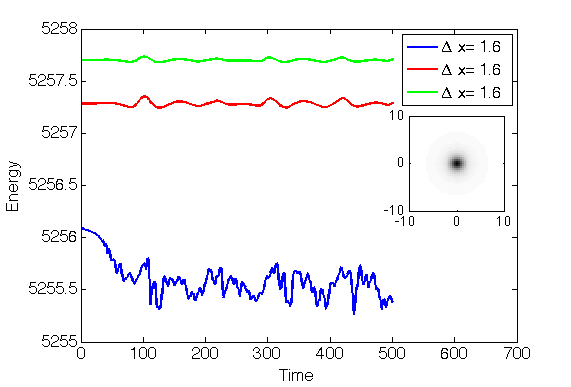
\includegraphics[width=0.5\textwidth]{numerics/figures/homg_energy_cons.png}
\end{figure}

\section{\label{section:vortexidentifying} Identifying vortices}
	\subsection{\label{section:gaussianblur} Image filters and the Gaussian kernel}
	\IncMargin{1em}
		\begin{algorithm}
		\SetKwData{Left}{left}\SetKwData{This}{this}\SetKwData{Up}{up}
		\SetKwFunction{Union}{Union}\SetKwFunction{FindCompress}{FindCompress}
		\SetKwInOut{Input}{Input}\SetKwInOut{Output}{Output}
		\Input{A field $P \in \mathbb{R}$ of size $nx \times ny$, a Gaussian filter size $g\in\mathbb{R}$, a line integral length $nl\in\mathbb{N}$.}
		\Output{A field $P \in \mathbb{R}$ of size $nx \times ny$ }
		\BlankLine
		\emph{special treatment of the first line}\;
		\For{$i\leftarrow 2$ \KwTo $l$}{
		\emph{special treatment of the first element of line $i$}\;
		\For{$j\leftarrow 2$ \KwTo $w$}{\label{forins}
		\Left$\leftarrow$ \FindCompress{$Im[i,j-1]$}\;
		\Up$\leftarrow$ \FindCompress{$Im[i-1,]$}\;
		\This$\leftarrow$ \FindCompress{$Im[i,j]$}\;
		\If(\tcp*[h]{O(\Left,\This)==1}){\Left compatible with \This}{\label{lt}
		\lIf{\Left $<$ \This}{\Union{\Left,\This}}\;
		\lElse{\Union{\This,\Left}\;}
		}
		\If(\tcp*[f]{O(\Up,\This)==1}){\Up compatible with \This}{\label{ut}
		\lIf{\Up $<$ \This}{\Union{\Up,\This}}\;
		\tcp{\This is put under \Up to keep tree as flat as possible}\label{cmt}
		\lElse{\Union{\This,\Up}}\tcp*[r]{\This linked to \Up}\label{lelse}
		}
		}
		\lForEach{element $e$ of the line $i$}{\FindCompress{p}}
		}
	\caption{disjoint decomposition}\label{algo_disjdecomp}
	\end{algorithm}\DecMargin{1em}

\section{\label{section:vortexclustering} Quantifying vortex clustering}
	\subsection{\label{section:reevesalgorithm} Recursive Cluster Algorithm (RCA) }
	\subsection{\label{section:ripleysk} Ripley's K function }
\section{\label{section:vortextracking} Tracking vortex trajectories}
\section{\label{section:vortexremoval} Removing vortices with ``phase unwrapping''}
	\IncMargin{1em}
	\begin{algorithm}
	\SetKwData{Left}{left}\SetKwData{This}{this}\SetKwData{Up}{up}
	\SetKwFunction{Union}{Union}\SetKwFunction{FindCompress}{FindCompress}
	\SetKwInOut{Input}{input}\SetKwInOut{Output}{output}
	\Input{A bitmap $Im$ of size $w\times l$}
	\Output{A partition of the bitmap}
	\BlankLine
	\emph{special treatment of the first line}\;
	\For{$i\leftarrow 2$ \KwTo $l$}{
	\emph{special treatment of the first element of line $i$}\;
	\For{$j\leftarrow 2$ \KwTo $w$}{\label{forins}
	\Left$\leftarrow$ \FindCompress{$Im[i,j-1]$}\;
	\Up$\leftarrow$ \FindCompress{$Im[i-1,]$}\;
	\This$\leftarrow$ \FindCompress{$Im[i,j]$}\;
	\If(\tcp*[h]{O(\Left,\This)==1}){\Left compatible with \This}{\label{lt}
	\lIf{\Left $<$ \This}{\Union{\Left,\This}}\;
	\lElse{\Union{\This,\Left}\;}
	}
	\If(\tcp*[f]{O(\Up,\This)==1}){\Up compatible with \This}{\label{ut}
	\lIf{\Up $<$ \This}{\Union{\Up,\This}}\;
	\tcp{\This is put under \Up to keep tree as flat as possible}\label{cmt}
	\lElse{\Union{\This,\Up}}\tcp*[r]{\This linked to \Up}\label{lelse}
	}
	}
	\lForEach{element $e$ of the line $i$}{\FindCompress{p}}
	}
	\caption{disjoint decomposition}\label{algo_disjdecomp}
	\end{algorithm}\DecMargin{1em}
\end{chapter}
